\chapter{\textit{Physarum polycephalum} Maintenance Protocol}
\label{chapter:protocol}
Observations of a living \textit{Physarum polycephalum} are the basis for the proposed algorithm. As even examination should be unbiased and repeatable. Therefore an appropriate set of procedures should be used. The authors have no background in microbiology or any related fields, which makes this task especially cumbersome. However, the methods presented here allowed the organism to survive for over 6~months, which was enough to make valuable observations. Such a long time included experiment sessions, each lasting for about a day or two, included in section \ref{ss:obervations}.


\section*{Storage}

The organism arrived safely on a Petri dish, which was placed inside a large transportation box, among other things. It was not affected by a long journey (from supplier Carolina Biological Supply,~USA to Poznan University of Technology,~Poland), even though it was X-rayed many times on its way to us. It was equipped with enough oatmeal food sources to survive such a journey (figure \ref{figure:p_initial_petri}).

On the day of arrival, as per hints from \cite{adamatzky2010physarum}, the organism was moved to a large plastic box, filled with a 2\%~non-nutrient~agar substrate (figure \ref{figure:p_box}). A large $20\times20$~cm surface of the box allowed \textit{Physarum polycephalum} to move freely, without any limitations. A thick layer of the substrate was enough for keeping the organism well moisted for about 12~weeks time. After that time the organism has been replanted to a similar box.

This box has been kept inside a shoebox, which created a perfectly dark environment for the organism. The box has been opened only when needed, minimizing the time of exposition of the slime mould to the light. Furthermore, when detailed observations or experiments had to be made, some of the plasmodium have been subcultured to an individual Petri~dish (figure \ref{figure:p_multiple_petri}). This minimized the influence of external conditions on the culture of \textit{Physarum polycephalum}, as it was still kept in the dark box.

The box has been placed in a shadow, with temperatures varying from 20~$^{\circ}$C to 25~$^{\circ}$C. Unfortunately, we were not able to stabilise the temperature more, as the experiments have been made at home.

\begin{figure}
  \centering

  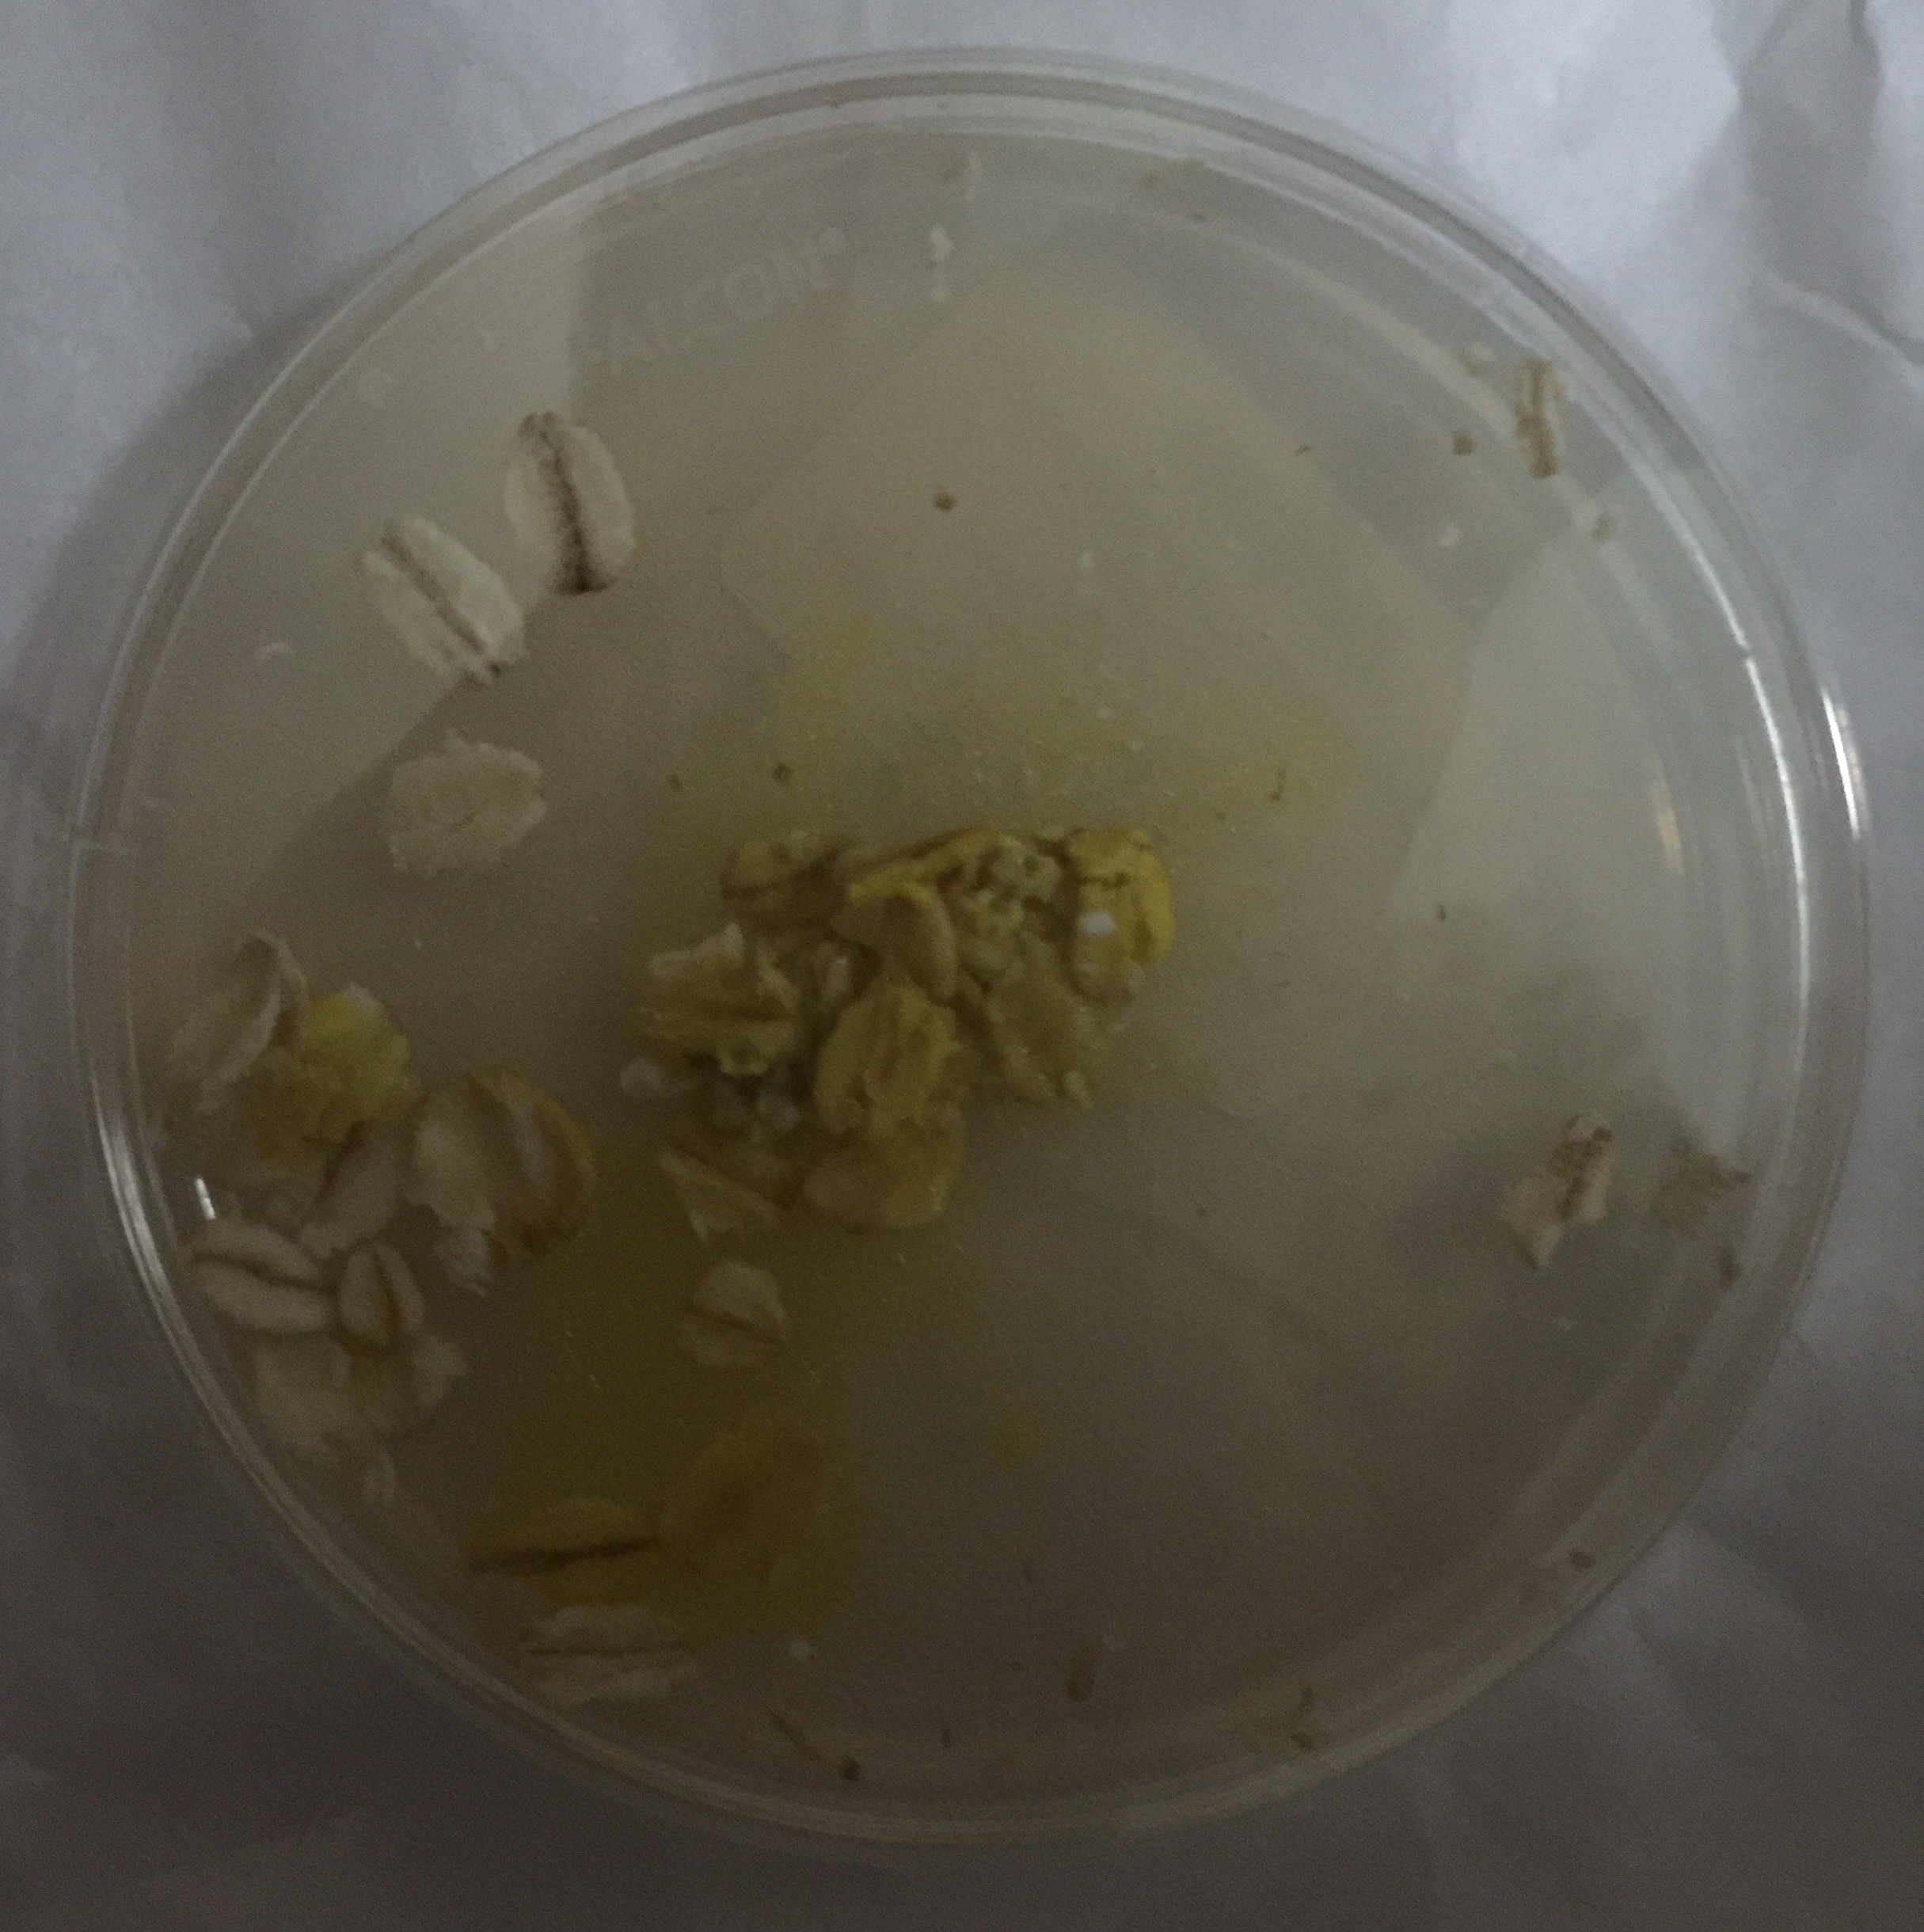
\includegraphics[width=0.8\textwidth]{figures/physarum/IMG_1168_crop.jpg}

  \caption{\textit{Physarum polycephalum} on its arrival}
  \label{figure:p_initial_petri}
\end{figure}

\begin{figure}
  \centering

  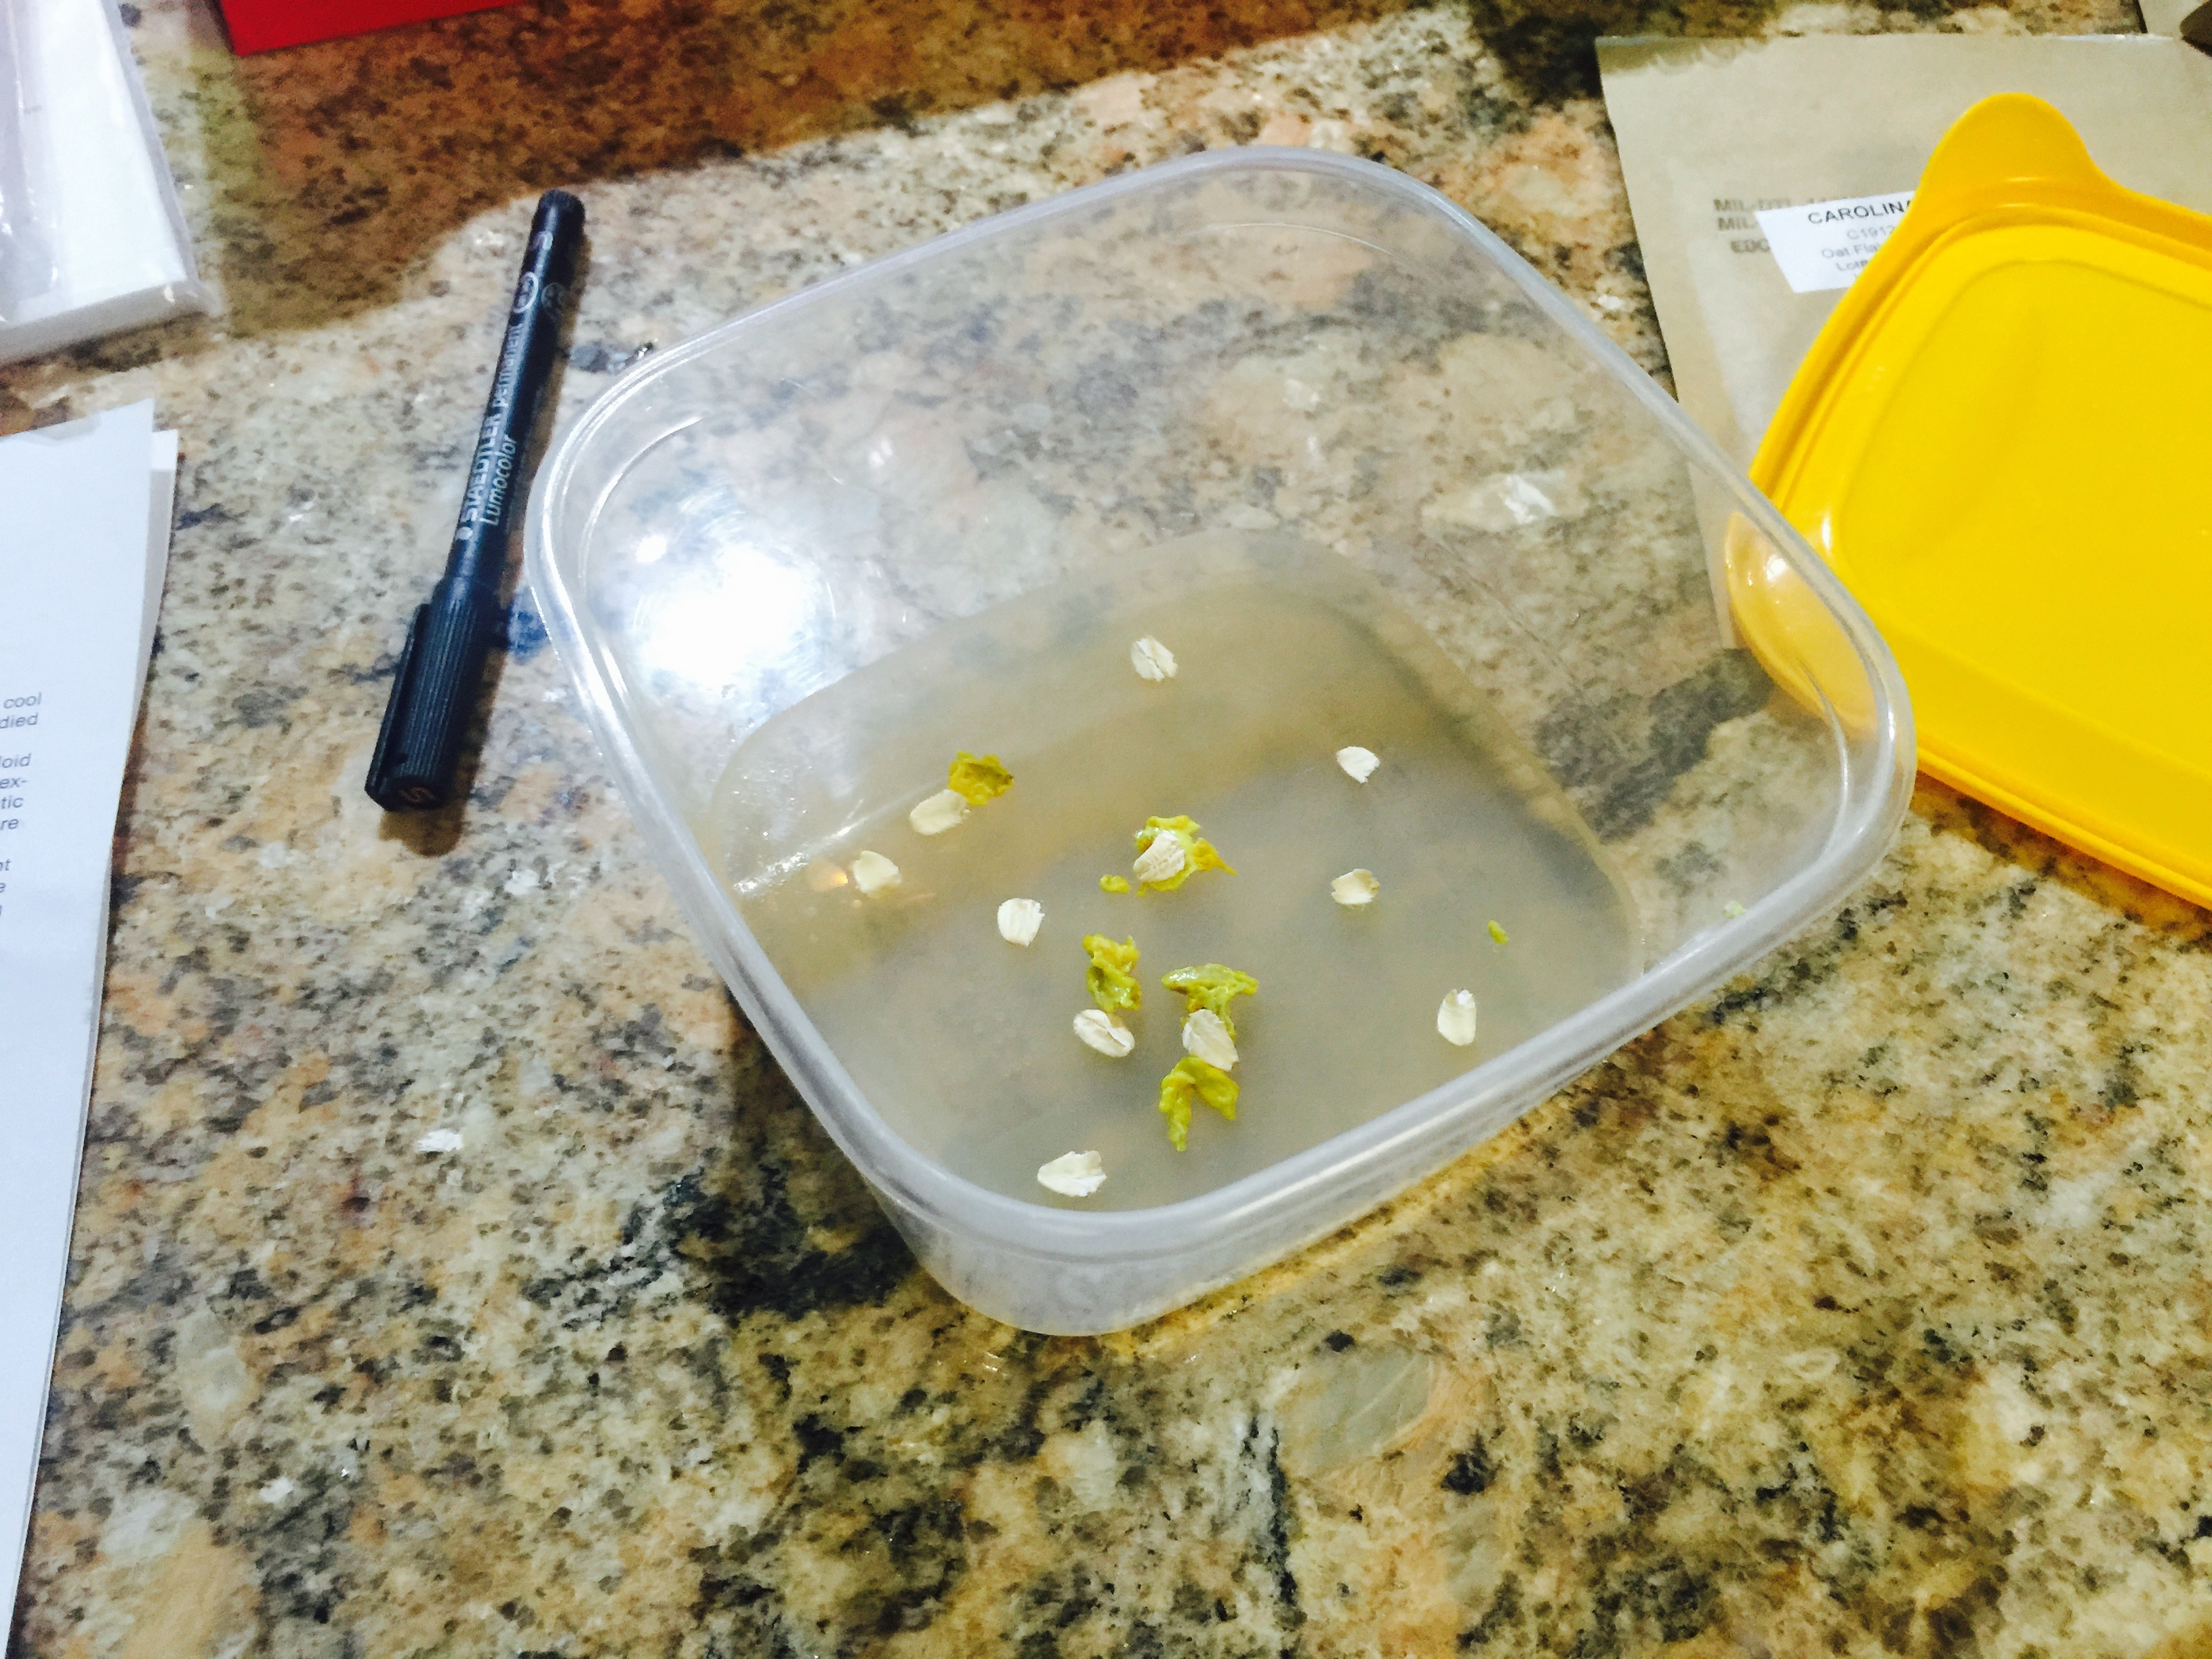
\includegraphics[width=0.8\textwidth]{figures/physarum/IMG_1179.jpg}

  \caption{The permanent storage box}
  \label{figure:p_box}
\end{figure}

\begin{figure}
  \centering

  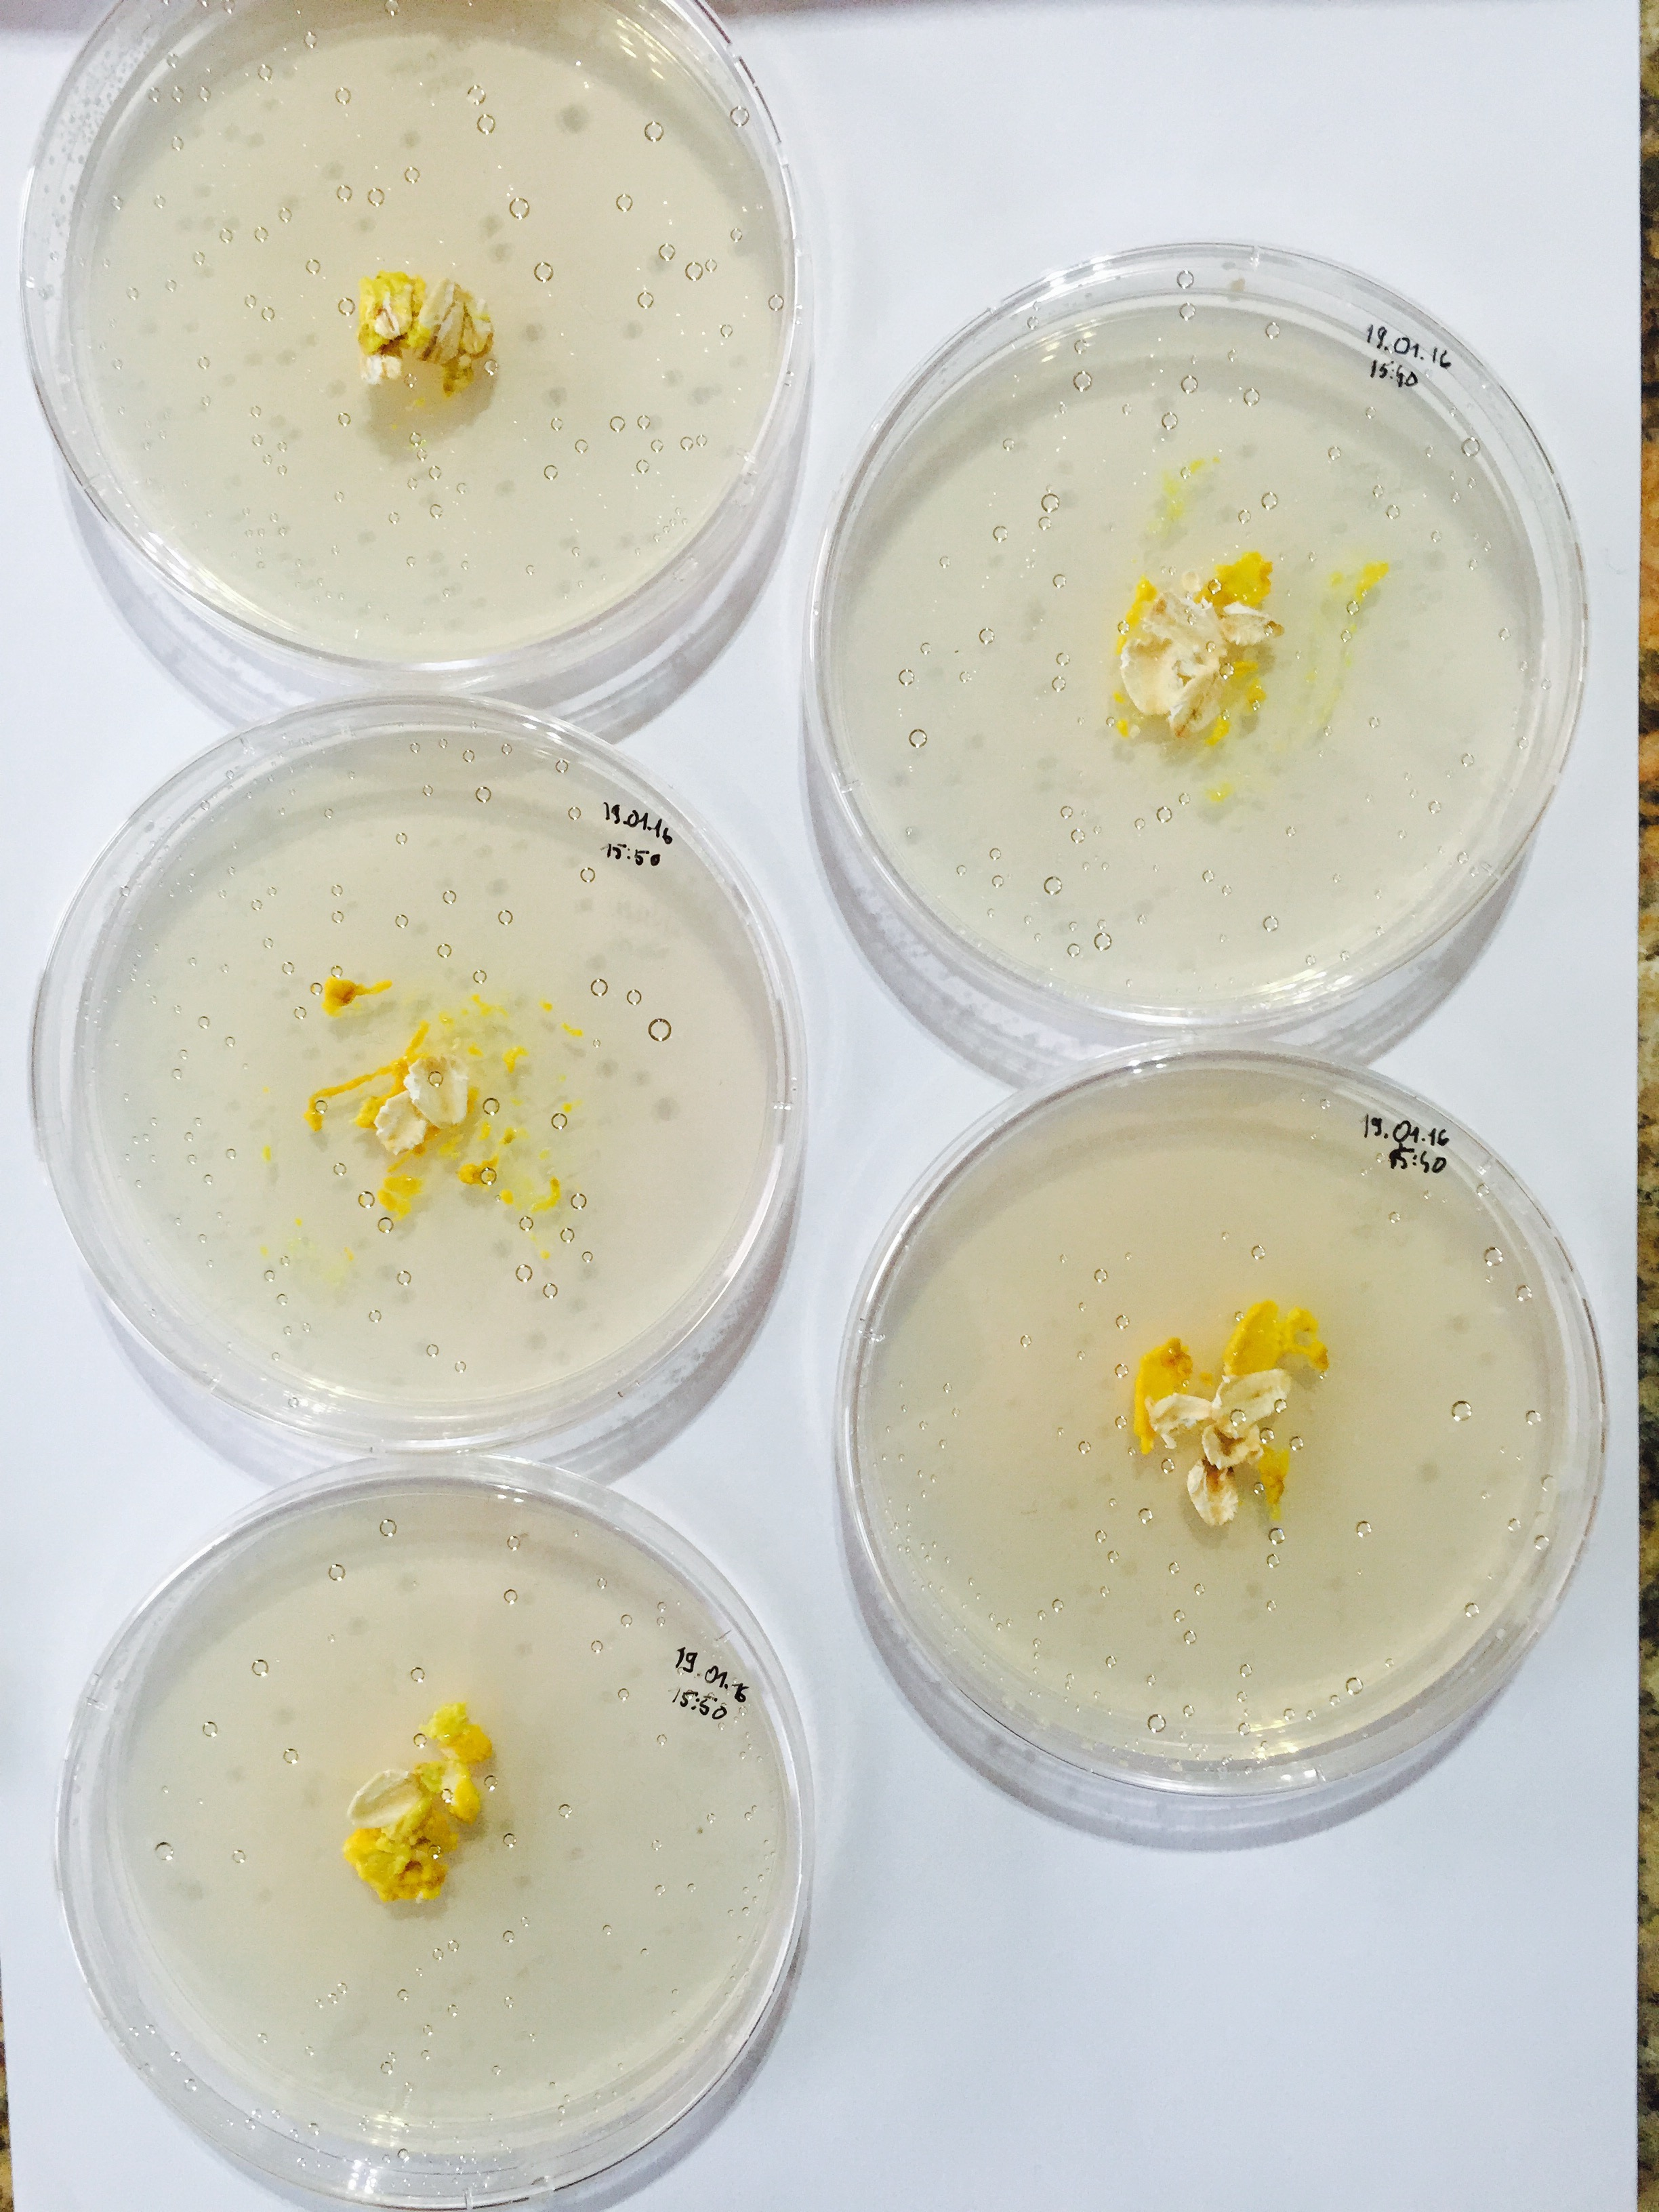
\includegraphics[width=0.75\textwidth]{figures/physarum/IMG_1175.jpg}

  \caption{Petri~dishes with a subcultured slime mould}
  \label{figure:p_multiple_petri}
\end{figure}


\subsection*{The substrate}

It is recommended by the supplier to cultivate \textit{Physarum polycephalum} on a sterile 2\%~non-nutrient~agar. The agar is a powder obtained from the algae, with an ability to bound water, while being neutral to many microorganisms (unlike gelatine). When it is mixed with water it creates a jelly-like substance which can be used as a substrate in Petri~dish. The supplier provided a few bottles of already prepared sterile agar substrate. However, in a room temperature it is a solid substance. The agar solution must be heated in order to be transferred to a Petri~dish or an other vesel. A common protocol recommends usage of a microwave oven \cite{hanson1978microwave} and it was used as a quick and practical solution to this problem.

When this premade substrate was exhauseted, we have created our solution of 2\%~non-nutrient~agar using an agar used for cooking and distilled water. We ensured to boil the solution for a while and stored it in preboiled bottles, therefore minimizing a chance of contamination, even though the solution was not truly sterile. This homemade solution compared to the premade substrate, made no observable difference in a behaviour of \textit{Physarum polycephalum}.


\section*{Nutrients}

Multiple sources recommend usage of sterile oatmeals as the main source of nutrients for the slime mould \cite{nakagaki2000intelligence,nakagaki2004obtaining,adamatzky2010physarum}. Initially some amount of sterile oatmeal has been provided by the supplier, however, it was quickly used up. The ecological, organic oatmeals have been bought and sterilised by cooking with distilled water. Such a porridge has been used as a main source of nutrients for \textit{Physarum polycephalum} (figure \ref{figure:p_porridge}).

\begin{figure}
  \centering

  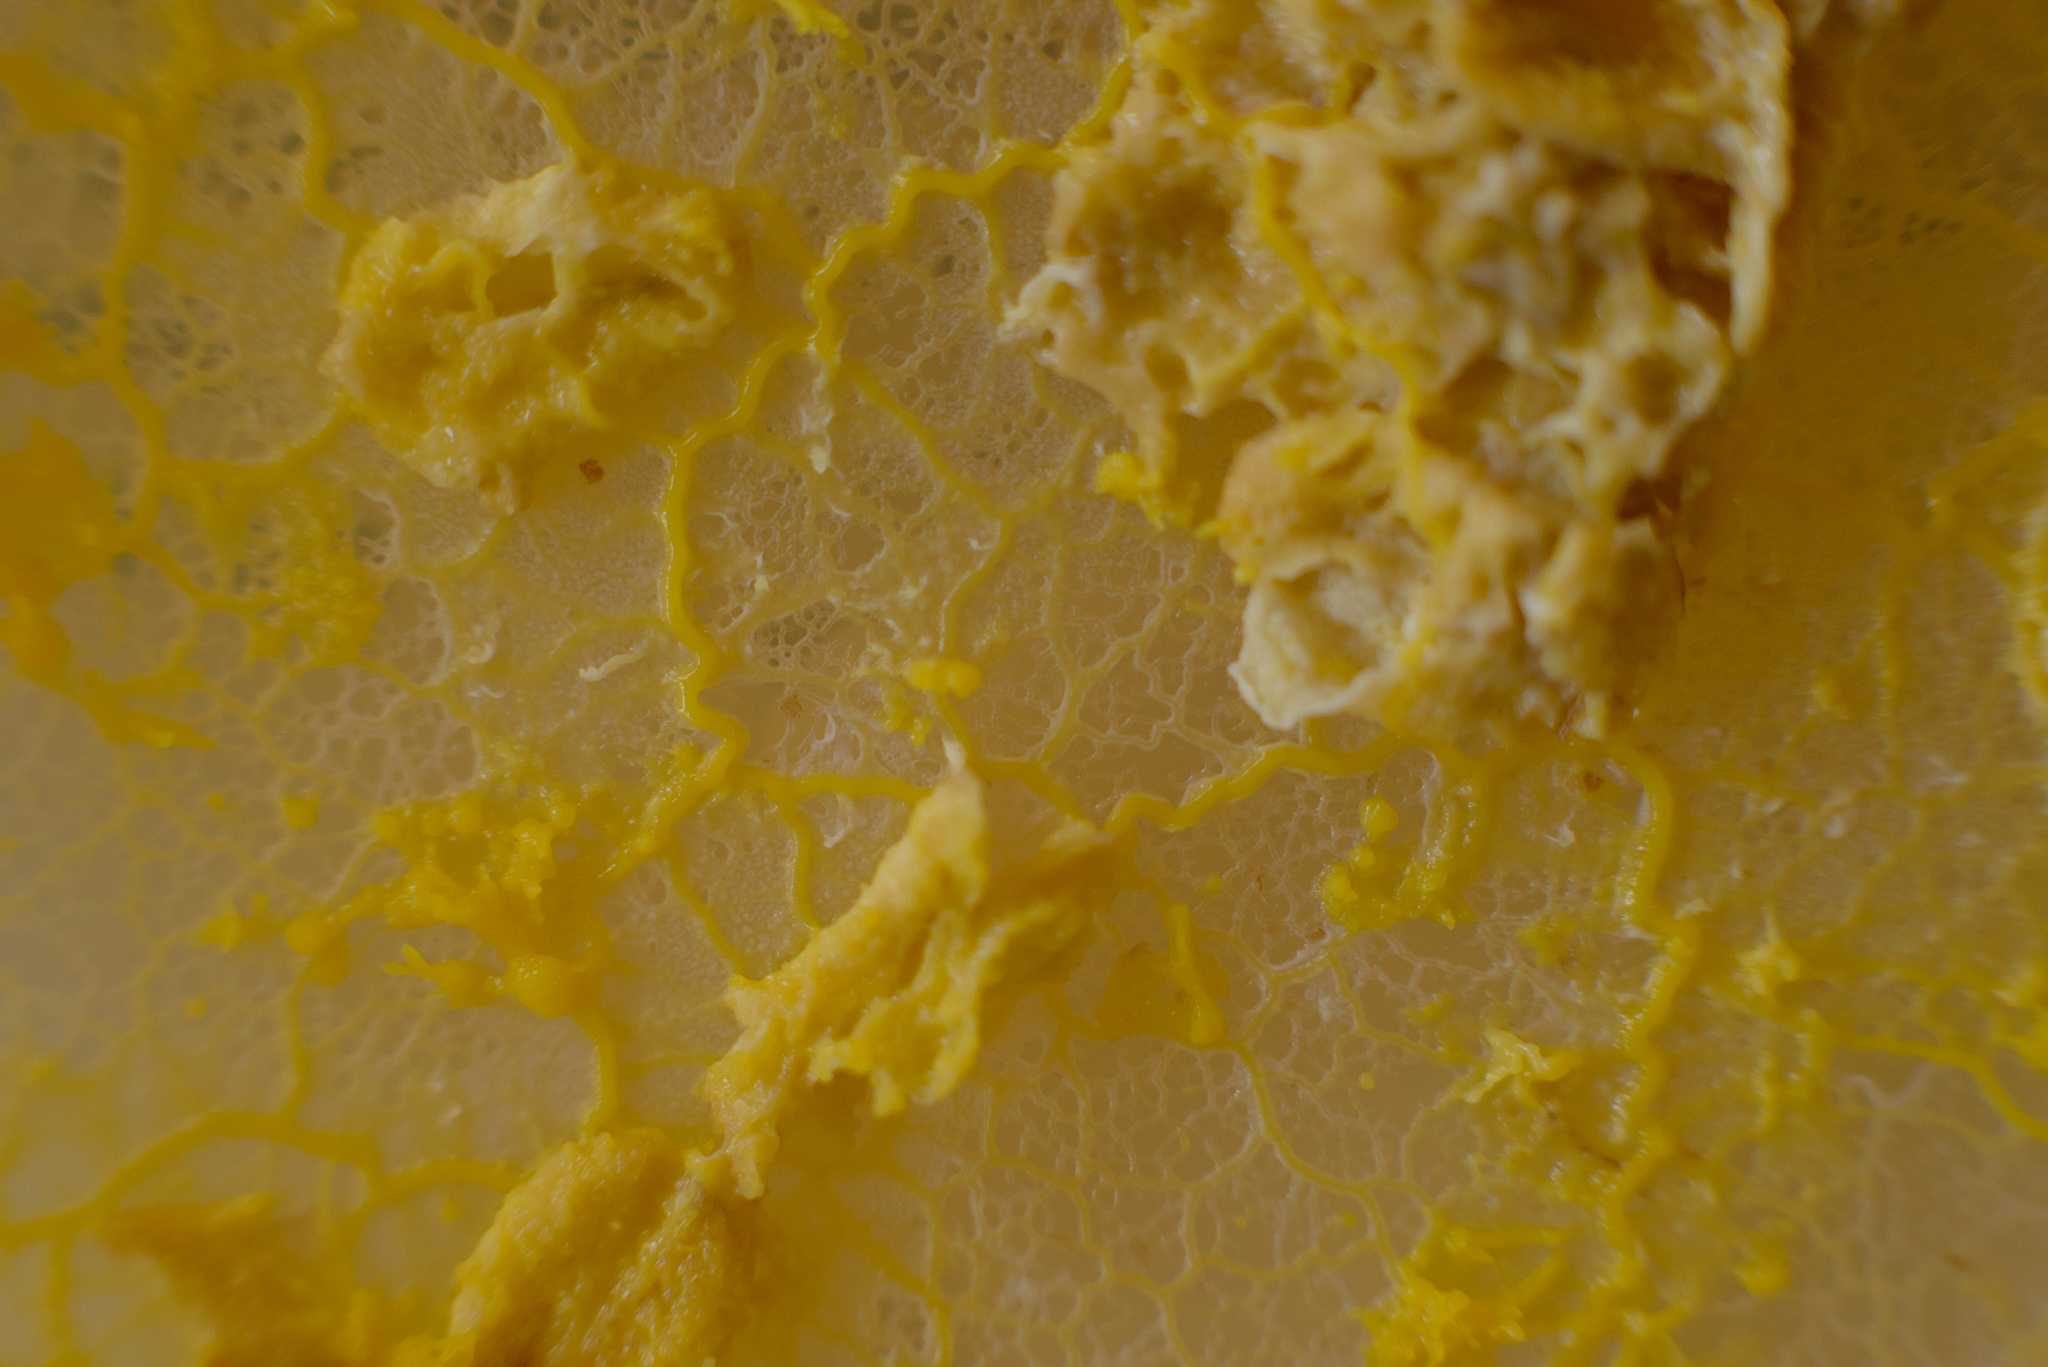
\includegraphics[width=0.8\textwidth]{figures/physarum/D8E_2184.jpg}

  \caption{\textit{Physarum polycephalum} foraging on an oatmeal porridge}
  \label{figure:p_porridge}
\end{figure}

Furthermore, a regular humidification was required to keep the organism in its plasmodial stage. A rule of thumb from \cite{adamatzky2010physarum} was used: ``If it's too mushy it's too dry, if it's too smelly it's too wet''. The organism has been sprayed with a distilled water when needed. When no distilled water was available, the tap water has been used, though it slightly affected the mobility of the slime mould.
